\chapter{分类指标}

\section{混淆矩阵}
混淆矩阵又称为错误矩阵,可以直观地观察到算法分类的效果。
它的每一列代表样本的预测分类,每一行代表样本的真实分类。
混淆矩阵i行j列的原始是原本是类别i却被分为类别j的样本个数,
计算完之后还可以对之进行可视化:
\begin{figure}[h]
    \centering
    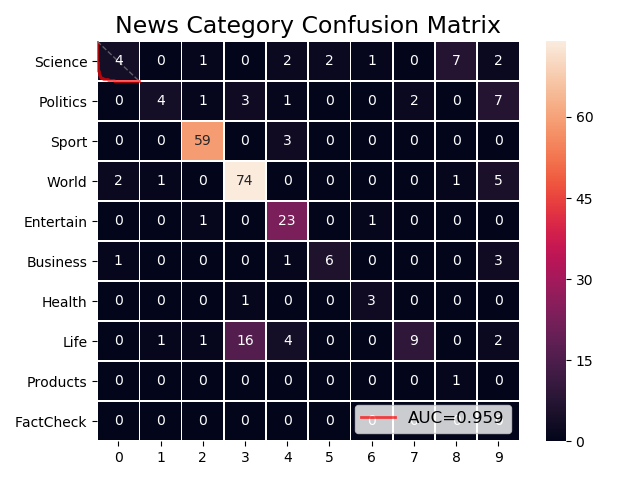
\includegraphics[width=9cm, height=6cm]{1_1.png}
    \caption{多元混淆矩阵}
\end{figure}

以二元分类为例来说,混淆矩阵如下:

\begin{figure}[h]
    \centering
    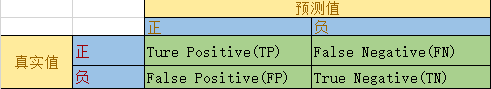
\includegraphics[width=12cm, height=2cm]{1_2.png}
    \caption{二元混淆矩阵}
\end{figure}

\begin{itemize}
    \item TP:真实结果为正,预测也为正
    \item FN:真实结果为正,预测也为负
    \item FP:真实结果为负,预测也为正
    \item TN:真实结果为负,预测也为负
\end{itemize}

\section{精确率和召回率}
